\documentclass[parskip=full,12pt,a4paper,twoside,headings=openright]{scrreprt}
% switch to scrbook if you want roman page numbers for the front matter
% however scrbook has no 'abstract' environment!
% if your thesis is in english, use "parskip=no" instead

% binding correction (BCOR) von 1cm für Leimbindung
\KOMAoptions{BCOR=1cm}
\KOMAoptions{draft=yes}

\usepackage[utf8]{inputenc} % encoding of sources\\
\usepackage[T1]{fontenc}
\usepackage{studarbeit}
\usepackage{algorithm2e}
\usepackage{pgfplotstable,filecontents}
\pgfplotsset{compat=1.9}% supress warning
%
\title{Verbesserte Optimierung von Integer-Konvertierungen und VHDL-Codeerzeugung mittels Bitbreitenanalyse}
\author{Marcel Hollerbach}
\thesistype{Bachelorarbeit}
\zweitgutachter{Prof.~Dr.~rer.~nat.~Bernhard~Beckert}% for verification stuff
%r\zweitgutachter{Prof.~Dr.-Ing.~Jörg~Henkel}% for compiler stuff
\betreuer{M.Sc. Andreas Fried}
\coverimage{4665389330_d09f3d6b75_z.jpg}

\newcommand{\libFIRM}{lib\textsc{Firm}}

\begin{document}

\begin{otherlanguage}{ngerman} % Titelseite ist immer auf Deutsch
\mytitlepage
\end{otherlanguage}

\begin{abstract}
\begin{center}\Huge\textbf{\textsf{Zusammenfassung}}
\end{center}
\vfill

Normal high level programming languages often just present standard data types for 8, 16, 32 and 64 bit numbers. However, the whole bandwidth of those data types is often not used at all. 

Looking at bigger C projects also shows that often enough C developers are using data types which are a lot bigger than there maximum number. \textit{integer} types are used as a standard complete number type in those projects. Instead of a smaller better fitting number type.
With the analysis presented in this work, the data types can be better adjusted to a good fitting data word length.
\vfill

In high-level Programiersprachen wie C gibt es vordefinierte Datentypen wie 8 / 16 / 32 / 64 bit Datentypen. Diese werden jedoch often nicht so eingesetzt das die moeglichst beste auslastung der moeglichen Zahlen erreicht wird.

Im hinblick auf C Projekte zeigt sich auch das der datentyp \textit{integer} immer mehr zu einem allgemein gueltigen Zahlendatentyp wird, welcher jedoch so gut wie nie die maximale groesse seiner zahlen erreicht.

In dieser arbeit geht es um die analyse, welche es erlaubt zu erkennen ob ein datentyp voll ausgenutzt wird oder nicht.

\todo{Das Titelbild ist von
\url{http://www.flickr.com/photos/x-ray_delta_one/4665389330/}
und muss durch ein zum Thema passendes Motiv ausgetauscht werden.}
\end{abstract}

\tableofcontents

\chapter{Introduction}\label{sec:intro}

Projects like \textit{libva} have made the first step into the direction of hardware accelerated video decoding on a computer system. These projects provide standardized access to decoding video streams like MPEG-2, H.264/AVC, H.265/HEVC, VP8, VP9, VC-1. The project itself handles the passing and messaging from a front end application like a video player, to the driver itself. The driver itself then answers the calls from the API. And the decoded picture goes back to the front end application. However, the driver itself still needs to do the decoding on its side. Usually implemented in hardware, since this is resulting in the best performance. The amount of work needed for implementing such a decoder for MPEG-2 can be observed while reading \cite{mpeg2-modelling}.
Thus it would be nice if software that gets written in C, can also be adopted to work directly on hardware. As an example, a C library which does decoding of MPEG-2 could just share its decoding code with a Hardware Description Language. There are techniques for doing this. However, they suffer from a lag of performance.
This thesis tries to improve the speed of such code by reducing the used bits of the software. The solution has two pieces, an analysis and a optimization.
The initial idea of the analysis is to annotate every operation with the bitwidth it requires. The following C snippet is formated a bit unlikely in order to make it easier to annotate.
\begin{lstlisting}[frame=single]
int arr[4];

for (int i = 0; i < 4; i++) {
  //i requires 3 bits
  int x = i*i; //x requires 6 bits
  int y = (i << 4); //y requires 7 bits
  int res = x + y; //res requires 8 bits
  arr[i] = res;
}
\end{lstlisting}
Every operation has a bitwidth. The bitwidth is the number of bits that is used by the operation, as maximum the modes amount of bits is used. The required bits per operation are annotated as comment after the operation.
How exactly the bitwidth of a operation is calculated will be covered in the later chapters.
The information gathered from the analysis is then used for optimizing the compiler output. The optimization here can happen at two layers. The compiler we use here can be used to output a hardware description language called VHDL. This output will be optimized to have a more compact memory layout.
The other compiler output is assembler output, which can also be optimized. If those optimizations are successful and really safe up resources can be found in the later sections.

\chapter{Basics}\label{sec:basics}

\section{cparser / libfirm}
Modern compilers are now developed for over half a century. Over the time a new structure has evolved. Compilers are split into three parts. The first part is called \textit{front end} and handles everything related to the language specific parts. The second part is called \textit{middle ware} and handles the abstract notation of code execution. The last part is called \textit{back end} and does the translation into something like assembler or java bytecode. As an example, cparser is handling the C specific tasks. The parsed c code is then translated into a control flow graph from $\libFIRM$, which is the middle ware. The $\libFIRM$ middle ware then also acts as back end and translates the control flow graph into assembler / java bytecode.

\paragraph{Control flow graph in \libFIRM} The interaction between the front and middle ware is based on a data structure similar to a control flow graph, it is called FIRM graph. A FIRM graph is a directed graph. Each node is a operation. Nodes can have operands. We say that a node always depends on another node, when there is a edge from the node to the other node. The FIRM graphs are also the base structure for analyzing the control flow of a software. Such a analysis is called control flow analysis. The nodes of the FIRM graph can have be categorized in different types: control flow, arithmetical operations, memory handing, constant expressing. A node is additionally placed in a block. A node is executed if all its operands have been executed. Or, if there are no operands, when its block is executed.
Another software that does the same thing is \textit{clang}, where the back end is handled by \textit{llvm}.
A more in detail explanation can be found in \cite{libfirm}. A more theoretical and abstracted introduction to control flow graphs can be found in \cite{control-flow-analysis}

\paragraph{Confirm nodes in \libFIRM}
In $\libFIRM$ there are several node types, one of them is called "Confirm" node. A Confirm node does not have a hardware representation. A confirm node has 2 operands. They are called value and bound, additionally a Confirm node has a relation. As relations $\not=$, $=$, $<$, $>$, $>=$, $<=$ are possible. 
Written as prefix notation we can say that the Confirm node gives the assertion that $\tau(value, bound)$ is true, where $\tau$ is the relation. This is useful for control flow analysis, as the Confirm nodes can indicate possible shortcuts with knowledge that is gained from other analysis.

\subparagraph{True / false Blocks}
\begin{figure}
	\centering
	\begin{tikzpicture}[scale=1.0, transform shape]
		\node[graph]{
			\begin{tikzpicture}[remember picture]
			\node[block] (startblock) {
				\begin{tikzpicture}
				\node[firm]    (cmp)        at ( 0,2) {Cmp};
				\node[control] (cond)       at ( 0,1) {Cond};
				\node[control] (false)      at (-1,0) {Proj};
				\node[control] (true)       at ( 1,0) {Proj};
				
				\draw[dataDependency]    (cmp.120)     -- ++(0,0.1) -| (-1, 3);
				\draw[dataDependency]    (cmp.60)      -- ++(0,0.1) -| ( 1, 3);
				\draw[dataDependency]    (cond)        --              (cmp);
				\draw[controlDependency] (false.north) -- ++(0,0.1) -| (cond.240);
				\draw[controlDependency] (true.north)  -- ++(0,0.1) -| (cond.300);
				\end{tikzpicture}
			};
			\node[block, anchor=north east] (left) at ($(startblock.south) + (-1,-0.5)$) {
				\begin{tikzpicture}
				\node[const] (c0) at (0,0) {true-block};
				\end{tikzpicture}
			};
			\node[block, anchor=north west] (right) at ($(startblock.south) + (1,-0.5)$) {
				\begin{tikzpicture}
				\node[const] (c1) at (0,0) {false-block};
				\end{tikzpicture}
			};		
			% Control dependencies
			\begin{scope}[every path/.style = {controlDependency}]
				\draw (left.north)  -- ++(0,0.2) -| (false);
				\draw (right.north) -- ++(0,0.2) -| (true);
			\end{scope}
	
			\end{tikzpicture}
		};
	\end{tikzpicture}
\caption{The construct that is called a upper bound compare node}
\label{fig:compare}
\end{figure}

A compare node in $\libFIRM$ has always a relation, 2 operands and 2 blocks. The compare node executes the true block, when the relation and operands are evaluating to true. The false block is executed otherwise. The structure is visualized in \autoref{fig:compare}

\paragraph{Interaction from front to back end}

\begin{figure}
	\centering
	\begin{lstlisting}[frame=single]
	#include <stdlib.h>
	#include <stdio.h>
	
	int main(int argc, char const *argv[]) {
	  printf("Hello Firm!");
	  return 0;
	}
	\end{lstlisting} 
	\caption{Sample source code}
	\label{code:workflow:example}
\end{figure}

As an example, we want to compile the program code from \autoref{code:workflow:example}.
First of all, the front end parses the given source code. The parsed code then is transformed into a abstract syntax tree (AST). The representation in the abstract syntax tree encodes the syntactical informations from the software. File contents like curly are encoded in the structure, and are not explicitly represented in the AST. \newline
After that the AST is transformed into a FIRM graph. \newline
At this point the front end handed the informations for creating a binary programm to the back end. However, the front end can now tell the back end to perform optimizations on the FIRM graph. In terms of C, this is often controlled with the -O{1,2,3} flags. \newline
After the optimizations have taken place, the binary files are written into a file, and the compiler call is finished.
\begin{figure}
	\centering
	\begin{tabular}{c | c c c c c c c c c}
		value & 7 & 6 & 5 & 4 & 3 & 2 & 1 & 0 \\
		\hline
		5     & 0 & 0 & 0 & 0 & 0 & 1 & 0 & 1 \\
		-2    & 1 & 1 & 1 & 1 & 1 & 1 & 1 & 0 \\
	\end{tabular}
	\caption{Number representation}
	\label{fig:numbers}
\end{figure}
\paragraph{Number representation}
So-called \textit{modes} are used in $\libFIRM$ to categorize data words. A mode specifies a length in bits. A data word can have a sort, this can be \textit{integer}, \textit{float}, \textit{reference}, \textit{data} and \textit{boolean}. For us, the only interesting type is the integer type, since this is the only type where we can compute bitwidth for now. Those integer-modes can be signed or unsigned. The length of the mode defines the maximum number. If it is signed, then it also defines the minimum number. Otherwise the minimum is just zero. The sign is encoded using two's complement. There are the following integer modes : 
%\textit{mode\_Bs}:
\textit{int8},
%\textit{mode\_Bu}: 
\textit{uint8},
%\textit{mode\_Hs}: 
\textit{int16},
%\textit{mode\_Hu}: 
\textit{uint16},
%\textit{mode\_Is}: 
\textit{int32},
%\textit{mode\_Iu}:
\textit{uint32},
%\textit{mode\_Ls}: 
\textit{int64},
%\textit{mode\_Lu}:
\textit{uint64},

As an example, in \autoref{fig:numbers} two numbers are displayed with its hardware representation.
The term \textit{mode} is used to describe integer-modes for the rest of this thesis.


\section{Software theory}

There are a few mathematical basics which are known to be useful for performing compiler analysis. The first basic is the lattice. The second basic is the fixed point iteration.

\subsection{Lattice}

A lattice is an algebraic structure. For a lattice $L=(V,\sqcup,\sqcap)$, there are the following rules:

\begin{itemize}
	\item $\sqcup: V \times V \rightarrow V$ returns the smallest element, that is bigger or equal than the two operands
	\item $\sqcap: V \times V \rightarrow V$ returns the biggest element, that is smaller or equal than the two operands
%	\item $\forall a,b \in V : \exists a \sqcup b \wedge \exists a \sqcap b$
	\item $\forall u,v \in V : u \sqcup ( u \sqcap v) = v \wedge u \sqcap ( u \sqcup v ) = v$
\end{itemize}

Additionally we add te requirement of $|V| \not= \infty$. This is not a requirement for lattices in general. However, for fixed point iterations this requirement is precise enough.

The element, which is the least of all elements is called $\bot$. The greatest of all is called $\top$. A lattice can also be written down as a Hesse diagram, which can be seen in \autoref{fig:lattice}

A more detailed introduction can be found in \cite{lattice_theory}.

\subsection{Fixed point iteration}
Fixed point iteration is a method for finding a $x$ where we know that $f(x)=x$. \newline
First of all we define $f: D \rightarrow D$. $f$ is monotone, additionally $|D|$ must be finite. We call $x \in D$ a fixed point if $f(x)=x$.
For iterating we start with the minimum of D. We define $y_0=f(min(D))$, $y_i=f(y_{i-1})$. With the requirements from above we can say: $\exists i \in N : y_i = y_{i-1}$. For further reading, please see \cite{fixed-point-iteration-basic}

%\paragraph{Prove}$f$ is continuous, this means $\forall x >= y: f(x) >= f(y)$. So we know that $f(x) = y$ where $y > x$. Or $f(x) = x$, which means that we found a fixed point. However, the first case can only happen a finite amount of times, since $|D| \not= \infty$. Thus there has to exist a fixed point.

\paragraph{Data flow analysis}
We can adapt the fixed point iteration to work on a CFG. For the following we define additionally:
\begin{itemize}
	\item CFG is called $G=(V,E)$
	\item The lattice we use is called $L$
	\item $f _{node}:L \rightarrow L$ is the function for iterating on a single node. $f _{node}$ is monotonous.
	\item $D$ is a set, where we can say that: $\forall d \in D: d = \{(0, v_0), ... , (n, v_n)\}$
	\item $f(d) := \{(id, \hat{v})| (id, v) \in d \wedge f _{node}(v) = \hat{v}\}$
\end{itemize}

We start the iteration with $d_{bot} := \{(0,\bot), ..., (n, \bot)\}$. At some point, while continuing the iteration, we will find a $\hat{d} = f(\hat{d})$. 

%\paragraph{Prove}: $|D|$ consists of every possible configuration. There is only a finite amount of elements in the lattice. Thus we can say that $|D|=2^m$. \newline
%We say $d_1 <= d_2 \equiv \forall (id_2, v_2) \in d_2: \forall (id_1, v_1) \in d_1 : v_2 >= v_1$. $f_{node}$ is continuous. \newline
%f being not continuous means $\exists x <= y: f(x) > f(y)$.
%This means that there has to be a $v_x \in x$ and $v_y \in y$, where $f_{node}(v_x) > f_{node}(v_y)$ even if $v_x <= v_y$, which is against the definition of $f_{node}$. Thus f has to be continuous.

\section{Software basic}
\subsection{Worklist algorithm}

A possible solution for implementing fixed point algorithms could be done by iterating the whole CFG everytime a node changes. However, this is quite wasteful, since we know that the state of a node only depends on the state of its operands. Therefore a algorithm called \textit{worklist algorithm} has evolved and can be found in \autoref{worklist}.

\begin{algorithm}[H]
	worklist := {CFG.Nodes}\;
	\While{worklist not empty}{
		node := worklist.pop()\;
		node\_changed := recalc(node)\;
		\If{node\_changed}{
			\ForEach{operand $\in$ node.operands}{
				\If{!worklist.contains(operand)}{
					worklist.appi jend(operand)	
				}
			}
		}
	}
	\caption{Worklist alogithm}
	\label{worklist}
\end{algorithm}

The base idea is to maintain a worklist which contains all nodes that are dirty. A node is considered dirty, when its operands have changed, but the node itself is not recalculated. Additional informations can be found at \cite{iterative-data-flow-analysis-revisited}
%http://cseweb.ucsd.edu/classes/sp00/cse231/report/node12.html
\chapter{Design \& Implementation}\label{sec:impl}

\section{Bitwidth analysis}
The analysis is a data flow analysis. The analysis attaches a $(int,boolean)$ tuple to every meaningful node. A node is considered meaningful is the node has a integer style mode. We will reference the first value as \emph{stable bits} and the second bit as \emph{is positive}.

\paragraph{Bit representation}
The stable bits are indicating how many bits are stable, and therefore not used.
The second value of the tuple indicates if the value will ever reach negative numbers or not. And thus indicate at least one stable bit at the highest position. However, the second value is only meaningful for modes that allow signs.

\paragraph{Range representation}
There is also a second way of interpreting the two values. The stable bits can define a minimum and maximum range. The maximum number is reached if the stable bits are just always zero. If the mode is signed and the node is not positive, then the minimum number is reached by assuming all stable bits are one. Otherwise the minimum range is 0. We can define the following min max definitions for the ranges:

$
max_{bitwidth}(x)=
\left\{
\begin{array}{l}2^{stable\_digits-1}-1\\2^{stable\_digits}-1\end{array}
\begin{array}{l} {mode.signed} \\ {Otherwise} \end{array}
\right.
$

$
min_{bitwidth}(x)=
\left\{
\begin{array}{l}2^{stable\_digits-1}\\0\end{array}
\begin{array}{l} {mode.signed and is_positive} \\ {Otherwise} \end{array}
\right.
$

\begin{figure}
	\centering
	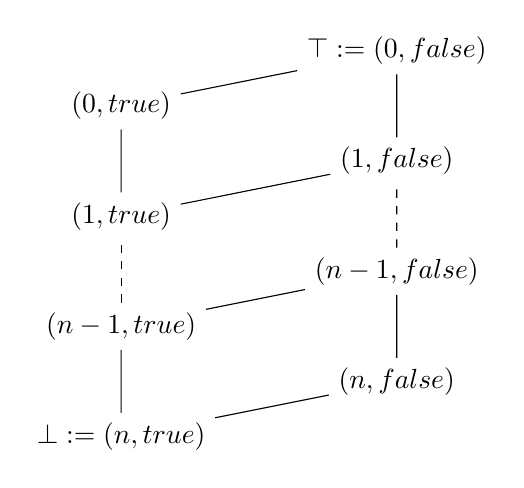
\begin{tikzpicture}[scale=.7]
		\node (np0) at(0,0) {$\bot := (n,true)$};
		\node (np1) at(0,2) {$(n-1,true)$};
		\node (np2) at(0,4) {$(1,true)$};
		\node (np3) at(0,6) {$(0,true)$};
		\node (p0) at(5,1) {$(n,false)$};
		\node (p1) at(5,3) {$(n-1,false)$};
		\node (p2) at(5,5) {$(1,false)$};
		\node (p3) at(5,7) {$\top := (0,false)$};
		\draw (np0) -- (p0) -- (p1) -- (np1) -- (np0);
		\draw (np2) -- (p2) -- (p3) -- (np3) -- (np2);
		\draw [dashed] (np1) -- (np2);
		\draw [dashed] (p1) -- (p2);
	\end{tikzpicture}
\caption{Hesse diagram of the lattice which is used in this analysis}
\label{fig:lattice}
\end{figure}

\paragraph{Analysis} The analysis works as a fixed point iteration. Therefore we use  \ref{fig:lattice} as lattice. The values of the lattice are representing the tuples from the analysis.

As a first step, we iterate over every single node and initialize the node with $\top$ and mark it as \textit{dirty}. If the node is constant, we calculate its bitwidth. Nodes with the opcodes \textit{Const}, \textit{Size} and \textit{Address} are considered constant.

The second step consists of recalculating every \textit{dirty} node in the graph. if $node.bitwidth < computed\_bitwidth$, the computed bitwidth is memorized as the new bitwidth of the node and every successor of the node is marked as dirty. The used rules for recalculating the nodes are described in REFERENCE TO TABLE %TODO.

\subsection{Definition: Value prediction}
In addition to the normal analysis results, the fixed point iteration can insert additional 
confirm nodes. Those confirm nodes help making the analysis more accurate.
First of all we need a few definitions for easier understanding:

\subparagraph{Definition: True / false Blocks}
%TODO

\subparagraph{Definition: Upper bounds}
\begin{figure}
	\centering
	\begin{tikzpicture}[scale=1.0, transform shape]
	\node[graph]{
		\begin{tikzpicture}[remember picture]
		\node[block] (startblock) {
			\begin{tikzpicture}
			\node[firm]    (predessors)       at (-1,3) {$\omega$};
			\node[const]    (c2)       at ( 1,3) {Const X};
			\node[firm]    (cmp)        at ( 0,2) {Cmp};
			\node[control] (cond)       at ( 0,1) {Cond};
			\node[control] (false)      at (-1,0) {False};
			\node[control] (true)       at ( 1,0) {True};
			
			\draw[dataDependency]    (cmp.120)     -- ++(0,0.1) -| (predessors);
			\draw[dataDependency]    (cmp.60)      -- ++(0,0.1) -| (c2);
			\draw[dataDependency]    (cond)        --              (cmp);
			\draw[controlDependency] (false.north) -- ++(0,0.1) -| (cond.240);
			\draw[controlDependency] (true.north)  -- ++(0,0.1) -| (cond.300);
			\end{tikzpicture}
		};
		\node[block, anchor=north east] (left) at ($(startblock.south) + (-1,-0.5)$) {
			\begin{tikzpicture}
			\node[const] (c0) at (0,0) {$\ominus$};
			\end{tikzpicture}
		};
		\node[block, anchor=north west] (right) at ($(startblock.south) + (1,-0.5)$) {
			\begin{tikzpicture}
			\node[const] (c1) at (0,0) {$\iota$};
			\end{tikzpicture}
		};		
		% Control dependencies
		\begin{scope}[every path/.style = {controlDependency}]
			\draw (left.north)  -- ++(0,0.2) -| (false);
			\draw (right.north) -- ++(0,0.2) -| (true);
		\end{scope}
		
	\end{tikzpicture}
};
\end{tikzpicture}
\caption{The definition of a upper bound compare node}
\label{fig:compare_upper_bound}
\end{figure}

A compare node is defining a upper bound if $node.relation = <$ and the node at $node.right$ is constant. For nodes where this is given we define
\emph{$\omega := node.left$} and the \emph{true block is called $\iota$}. A visualization of the definition is given at \ref{fig:compare_upper_bound}.
A compare node is also defining a upper bound if it can be transformed into a construct that matches the definition. For example with switching the right and left nodes, while turning the relation.
\subparagraph{Definition: Predecessor in a certain block}
\begin{center}
$\phi(a, b) := \forall X \prec a \wedge X.block = b$ 
\end{center}
$\phi$ returns every node that is a direct predecessor of a and located in block b.
\subparagraph{Definition: Constant dependencies}
\begin{center}
$\xi(a) := 
\left\{
	\begin{array}{l}
		a \cap \xi(c)\\ 
		\emptyset
	\end{array}
	\begin{array}{l}
		, \text{If there is only one not constant dependency \textit{c}} \\ 
		, \text{otherwise}.
	\end{array}
\right.$
\end{center}

If \textit{a} has only one not constant dependency node c, then $\xi$ returns the element a and $\xi(c)$. Otherwise it returns a empty set.

\paragraph{Upper bounds for block execution}
The values that are calculated in a node are (even if the fixed point iteration is not stable yet) possible values. The iteration starts at $\top$ and moves into the direction of $\bot$. This means that our range of possible values starts at something like $[0,0]$, moving towards $[n,-n]: n > 0 n <= max(mode)$ with each iteration. For a $\omega$ node this means that there can be a a recalculation, (new and old bitwidth is notated as the value range $\hat{x}$ and $x$) where the compare relation is true for $x$ but not anymore for  $\hat{x}$. This means that $\hat{x}$ is the upper bound for $\iota$. Thus we can insert a confirm node between every node $e \in \phi(\omega, \iota)$ and $\omega$.

\paragraph{Moving upper bounds backwards}
The confirms we have inserted between $\omega$ and its successors are not the only thing we can insert. We can also insert a confirm node between every $\phi(\xi(\omega), \iota)$. Important here is, the predecessors of $\omega$
Those confirms are then also inserted above conversation nodes, which is not possible using the normal construct insertion code provided by \libFIRM


\subsection{Difference to VRP}

There is already a analysis that is doing something similar, it is called value range propagation. The difference from VRP to BA is that in VRP each iteration is trying to predict the exact range after each operation. While BA tries to predict the unused bits after each operation. This little detail is mainly showing up in speed of the fixed point iteration, VRP converges way slower than BA. Details for this are given in the evaluation chapter \ref{sec:eval}.

\section{Stable Conversion nodes}
A conversion of a data word can result in two different results. First the bitwise representation stays the same. Second, the bitwise representation also gets mapped.
We call the first case \textit{Stable Conversion node}.

\paragraph{Finding stable conversion nodes}
Stable conversion nodes can be found using the bitwidth analysis. As described before, the analysis maps every node in the tree to a tuple. First number is the number of stable bits, which describes a upper bound for the numbers that will be written into the data word. The second number is a boolean flag and indicates if the number is going to be greater than 0 or not. If we now can see that the number range from the successor is the same as the one of the conversion node, then we can declare the conversion as stable.

\paragraph{Removing conversion nodes}
In case we found a stable conversion node, then we can say that this node only exists for syntax rules, there is no semantical value in them. Removing those nodes also has the advantage of helping other analysis. The confirm insertion algorithm of \libFIRM is searching for assertions that can be made based on looking at compare nodes. This works quite well. However, a construction like TODO does not work.
%FIXME diagram 
%FIXME reason
After removing the conversion node, the analysis can find a assertion based on the compare node. This also helps the branch prediction, dead code elimination. \newline
However, for really removing the conversion nodes, we need to find situations where we can eliminate the conversion node. One was already seen in the example. A compare node with a constant node as second operand. Another situation is a arithmetical operation with a constant and conversion node as operands.

\paragraph{Compare-Conversion optimization}
%FIXME diagram
\paragraph{Arithmetical-Conversion optimization}
%FIXME diagram
\chapter{Evaluation}\label{sec:eval}

Hier wird nun das Ergebnis des vorherigen Kapitels kritisch betrachtet.
Verbesserungen werden anhand von konkreten Experimenten und Zahlen belegt.
Eine saubere statistische Auswertung ist das Ziel.

Für schöne Tabellen ist das \enquote{booktabs} package zu empfehlen.
Ein Beispiel ist in \cref{fig:example_table} zu sehen.

\begin{figure}[hb]
\begin{center}
\begin{tabular}{lrrrr}
\toprule
Fach & xkcd Comics & Spaß & $\sigma$ & p \\
\midrule
Informatik & 1325 &  100\% & 12,3 & 3\% \\
Physik     & 1324,31 &  87\%& 1,733 & 0.03\%  \\
Geologie & 123 & 23\% & 1,3 & 11\% \\
Wirtschaft & 5 & 4\% & 12 & 1\% \\
Deutsch & 0 & 101 & 92,3 & 33\% \\
\midrule
Geom. Mittel & 743 & 63\% & 12,3 & 3\% \\
\bottomrule
\end{tabular}
\end{center}
\caption{Eine Beispieltabelle.
Man beachte, dass zwischen Datenzeilen keine Linien sind.
Außerdem ist der Beschreibungstext hier sehr ausführlich,
damit der Leser nicht den zugehörigen Abschnitt im Fließtext finden muss.
}
\label{fig:example_table}
\end{figure}

Zum Benchmarken empfehlen wir das Tool \enquote{temci}~\cite{temci} und ein Studium der zugehörigen Bachelorarbeit~\cite{bechberger16bachelorarbeit}.

\chapter{Conclusion}\label{sec:conclusion}

\section{Assembler generation}
The previous chapter showed that the optimizations are not that helpful on decoder code. This thesis was done for evaluating decoder code, so no others projects have been checked. However, other projects like direct UI or CLI implementations also could be evaluated, since the patterns from decoding code are quite different to ui codes. Without evaluating others, we can say, that the optimization for dropping conversion nodes from the graph is not that helpful.

\section{vhdl generation}

\section{Further improvements}

\section{Additional analyzer usage}

\bibliographystyle{ieeetr}
\bibliography{bib}

\begin{otherlanguage}{ngerman}
\chapter*{Erklärung}
\pagestyle{empty}

  \vspace{20mm}
  Hiermit erkläre ich, \theauthor, dass ich die vorliegende Bachelorarbeit selbst\-ständig
verfasst habe und keine anderen als die angegebenen Quellen und Hilfsmittel
benutzt habe, die wörtlich oder inhaltlich übernommenen Stellen als solche kenntlich gemacht und
die Satzung des KIT zur Sicherung guter wissenschaftlicher Praxis beachtet habe.
  \vspace{20mm}
  \begin{tabbing}
  \rule{4cm}{.4pt}\hspace{1cm} \= \rule{7cm}{.4pt} \\
 Ort, Datum \> Unterschrift
  \end{tabbing}
\end{otherlanguage}

\pagestyle{fancy}
\appendix

\chapter{Appendix}

\section{Table of node rules}

\label{table_of_rules}

A operation has operands, all of them are referred to as \textit{operands}, the first is called \textit{a}, the second is called \textit{b}. In the first column the formula for the new stable digits is displayed. The second column is the formula for the is\_positive flag. $n_{stable}$ is used in the second column to refer to the value calculated in the first column.

\begin{tabular}{ l | c | c }
	op & used bits & is\_positive \\
	\hline
	add & $max(min(a_{stable}, b_{stable}) - 1, 0)$ & $a_{positive} \wedge b_{positive} \wedge n_{stable} > 0 $\\
	minus &  $max(a_{stable} - 1, 0) $ & $\textit{false}$\\
	sub &  $max(min(a_{stable}, b_{stable}) - 1, 0) $ & $\textit{false}$\\
	mul &  $max(b - mode + a_{stable}, 0)  $ & $a_{positive} \wedge b_{positive} \wedge n_{stable} > 0 $\\
	div &  
	$ 
	\left\{
	\begin{array}{l}
	a_{stable}\\ 
    max(a_{stable} - 1, 0)
	\end{array}
	\begin{array}{l}
	, mode\text{ is signed} \\ 
	, \text{otherwise}.
	\end{array}
	\right.$
	& $a_{positive} \wedge b_{positive} \wedge n_{stable} > 0 $ \\
	mod &  & \\
	\hline
	shl & $a_{stable} - b_{stable}  $& 
	$ 
	\left\{
	\begin{array}{l}
	a_{positive}\\ 
	\text {false}
	\end{array}
	\begin{array}{l}
	, n_{stable} > 0 \\ 
	, \text{otherwise}.
	\end{array}
	\right.$
	 \\
	shr & $a_{stable} + b_{stable}  $& $\textit{true}$\\
	shrs & $a_{stable} + b_{stable}  $& $a_{positive}$\\
	\hline
	conv &  $ max(a_{stable} + (mode - old\_mode), 0)  $ & $a_{positive} \wedge n_{stable} > 0 $\\
	\hline
	$
	\begin{array} {l}
        \text{max} \\
        \text{phi} \\
        \text{and} \\
        \text{eor} \\
        \text{or} \\
	\end{array}$ & $min(operands)$ & $\bigwedge(operands_{positive})$ \\
	\hline
\end{tabular}

\end{document}
